\chapter{Os dentes e o comer bem}\label{ch:g2:teeth-and-eating-well}

Dê uma mordida numa maçã e olhe a marca: uma fileira curva e
caprichada de marquinhas. Foram os seus dentes --- uma caixa de
ferramentas completa que corta, rasga e tritura cada refeição antes
de você engolir. E, como toda boa caixa de ferramentas, ela merece
cuidado e coisas boas para trabalhar.

\begin{omfigure}
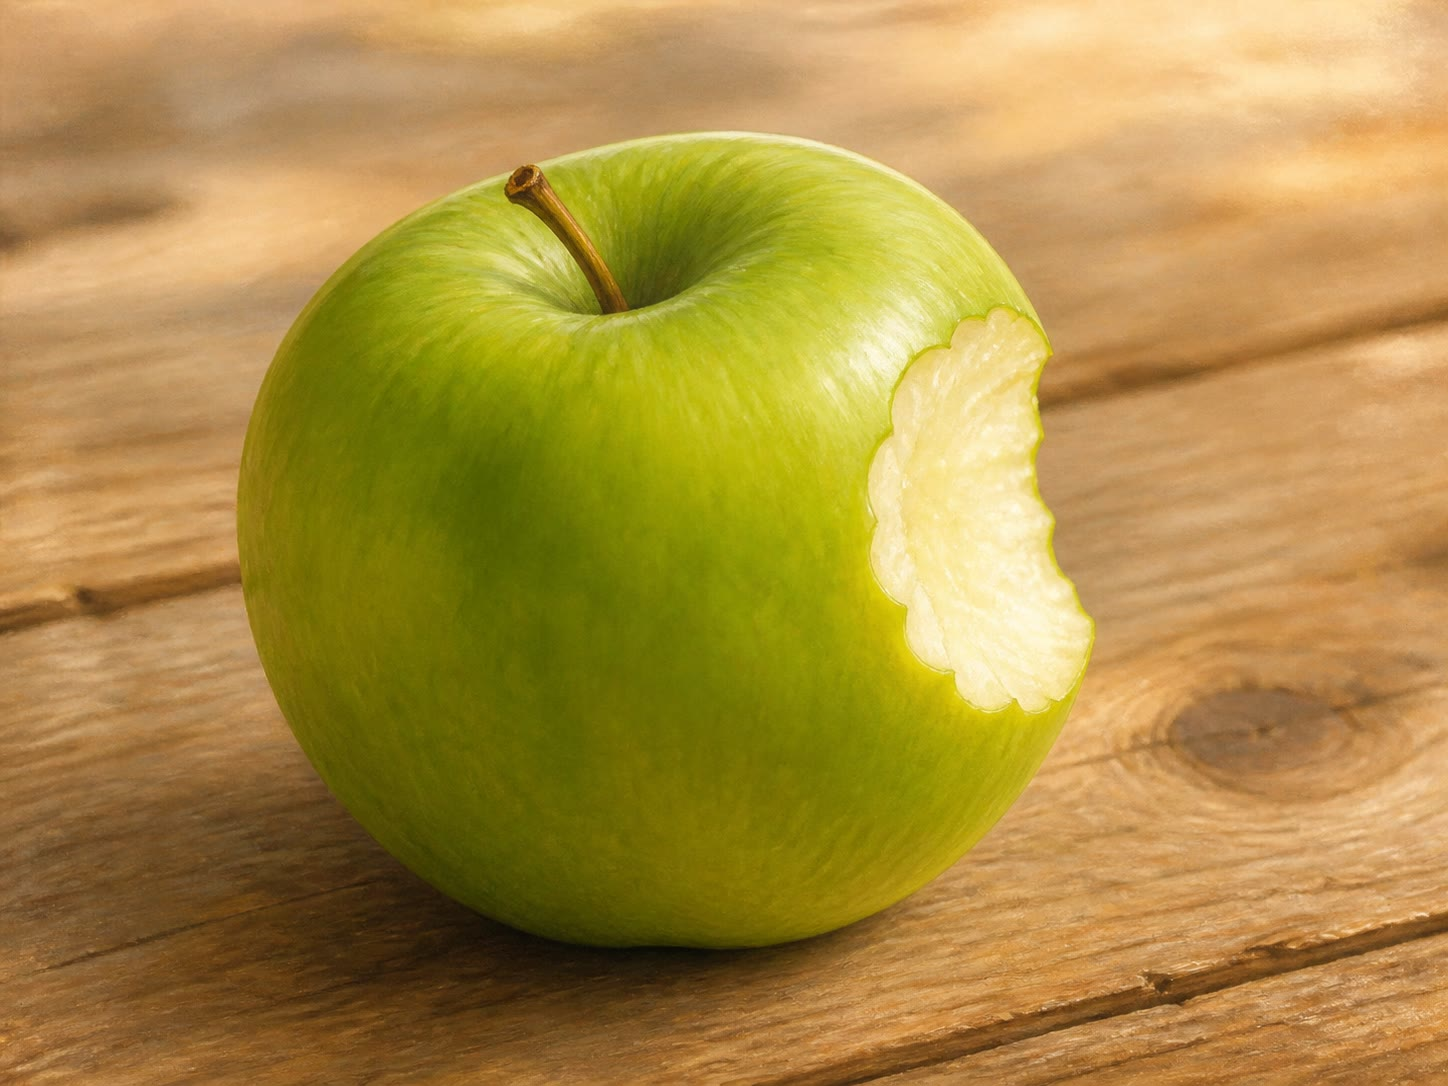
\includegraphics[width=0.55\linewidth]{images/book1/ai/g2-teeth-apple.jpg}

{\small A primeira prova do capítulo: uma mordida e a assinatura
curva e caprichada dos \omterm{def:g2:teeth-and-eating-well:kinds}{incisivos}.}
\end{omfigure}

\section{Os dentes: uma caixa de ferramentas na boca}

\begin{definition}[Os três tipos de dentes]\label{def:g2:teeth-and-eating-well:kinds}
Os dentes humanos vêm em três tipos, cada um com o seu trabalho:
\begin{enumerate}
  \item os \emph{incisivos}\index{incisivo}, chatos e afiados, na
        frente, \emph{cortam} --- eles fatiam a maçã;
  \item os \emph{caninos}\index{canino}, pontudos, nos cantos,
        \emph{rasgam} --- eles agarram e puxam os alimentos mais
        duros;
  \item os \emph{molares}\index{molar}, largos e cheios de
        saliências, no fundo, \emph{trituram} --- eles esmagam o
        alimento até virar uma pasta pronta para engolir.
\end{enumerate}
\end{definition}

\begin{omfigure}
\begin{tikzpicture}
  \node[anchor=south west, inner sep=0] (img) at (0,0)
    {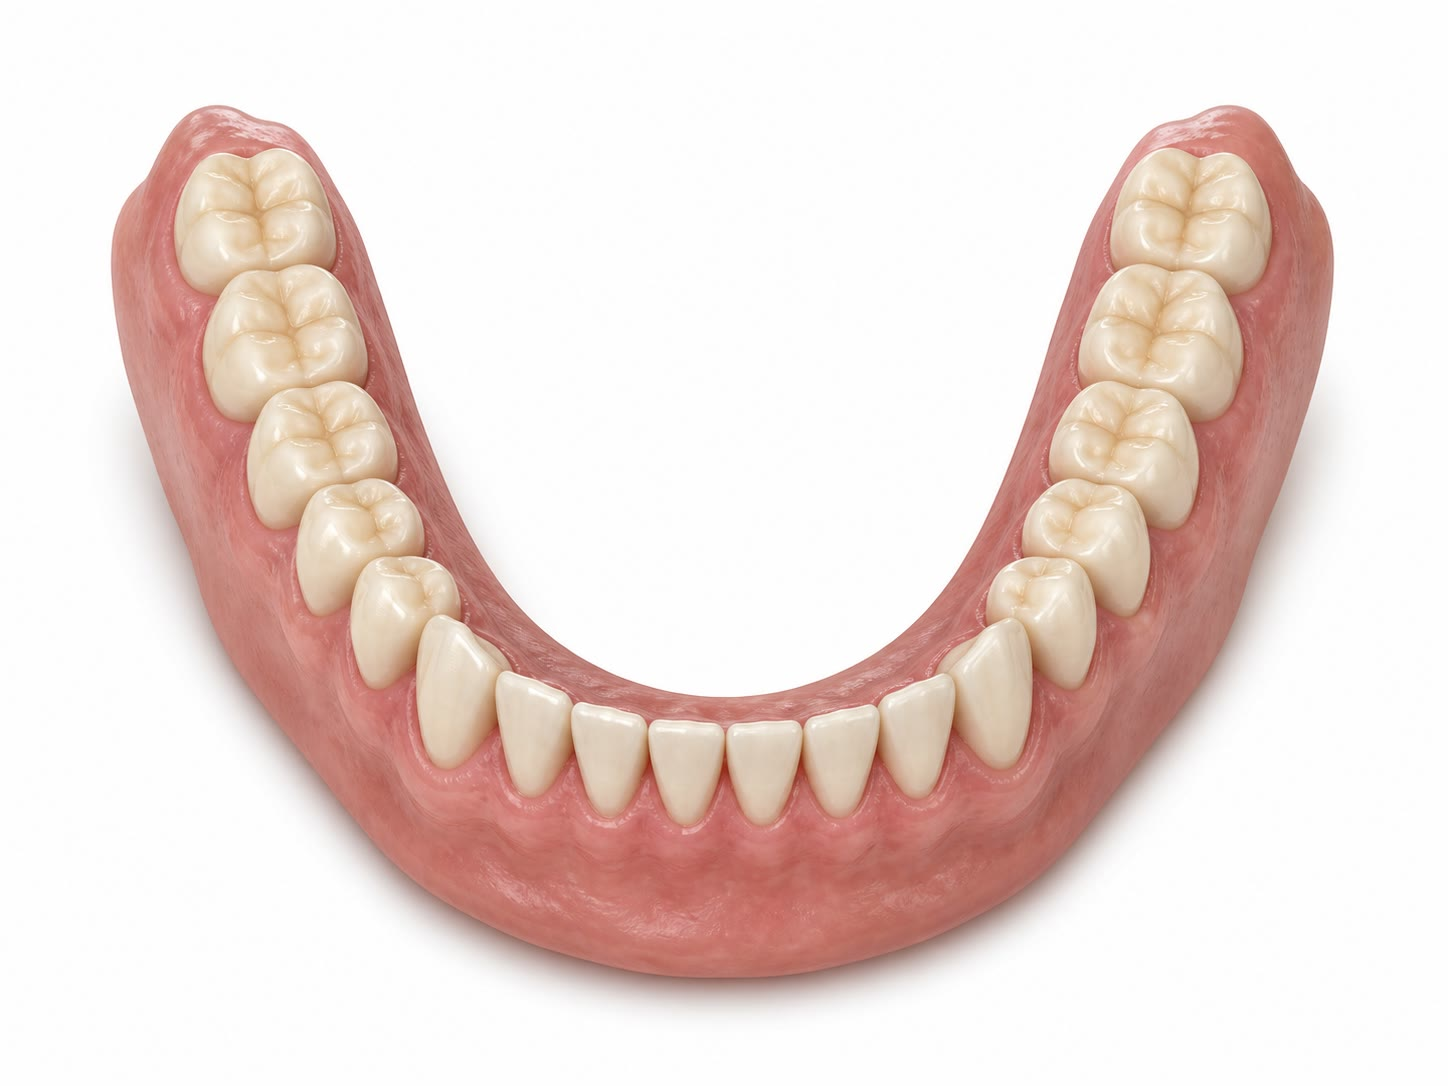
\includegraphics[width=0.56\linewidth]{images/book1/ai/fig-jaw-teeth.jpg}};
  \begin{scope}[x={(img.south east)}, y={(img.north west)},
      every node/.style={font=\small}]
    \draw[omDef, thick] (0.50,0.28) -- (0.50,0.06)
      node[below] {incisivos: cortam};
    \draw[omThm, thick] (0.31,0.44) -- (-0.03,0.40)
      node[left, align=right, omThm] {caninos:\\ rasgam};
    \draw[omMeth, thick] (0.80,0.72) -- (1.03,0.72)
      node[right, align=left, omMeth] {molares:\\ trituram};
  \end{scope}
\end{tikzpicture}

{\small A arcada de baixo: \omterm{def:g2:teeth-and-eating-well:kinds}{incisivos} que cortam na frente, \omterm{def:g2:teeth-and-eating-well:kinds}{caninos}
que rasgam nos cantos, \omterm{def:g2:teeth-and-eating-well:kinds}{molares} que trituram no fundo.}
\end{omfigure}

\begin{example}[Uma mordida de maçã, três ferramentas]\label{ex:g2:teeth-and-eating-well:apple}
Comer um pedaço de maçã usa a caixa de ferramentas inteira, em
ordem: os \omterm{def:g2:teeth-and-eating-well:kinds}{incisivos} fatiam a mordida, os \omterm{def:g2:teeth-and-eating-well:kinds}{caninos} ajudam a soltar o
pedaço e a língua leva tudo para trás, até os \omterm{def:g2:teeth-and-eating-well:kinds}{molares}, que trituram.
Só então você engole.
\end{example}

\begin{remark}[Lembre-se dos animais]\label{rem:g2:teeth-and-eating-well:animals}
A sua caixa de ferramentas misturada conta uma história: cortadores
e trituradores chatos como os de um \omterm{def:g2:what-animals-eat:kinds}{herbívoro}, \omterm{def:g2:teeth-and-eating-well:kinds}{caninos} pontudos como
os de um \omterm{def:g2:what-animals-eat:kinds}{carnívoro}. É a boca de um \omterm{def:g2:what-animals-eat:kinds}{onívoro} --- os seres humanos são
equipados para \omterm{def:g1:plants-around-us:plant}{plantas} \emph{e} carne, exatamente como o
\cref{ch:g2:what-animals-eat} nos classificou.
\end{remark}

\section{Dentes de leite, dentes de adulto}

\begin{proposition}[Duas dentições numa vida]\label{prop:g2:teeth-and-eating-well:sets}
Os seres humanos têm duas dentições. Os $20$ \emph{dentes de
leite}\index{dentes de leite} chegam nos primeiros anos de vida. Por
volta dos seis anos eles amolecem e caem um a um, empurrados de
baixo pelos \emph{dentes de adulto}\index{dentes de adulto} --- a
dentição final, de até $32$ dentes, que precisa durar o resto da
vida.
\end{proposition}
\admitted

\begin{example}[O incisivo bambo]\label{ex:g2:teeth-and-eating-well:wobbly}
Um dente da frente começa a ficar bambo justamente na idade em que
as crianças entram na escola. Embaixo dele, um \omterm{def:g2:teeth-and-eating-well:kinds}{incisivo} de adulto
vinha crescendo em silêncio e dissolvendo a \omterm{def:g1:plants-around-us:parts}{raiz} do dente de \omterm{def:g2:animals-grow-up:born}{leite},
até o dentinho se soltar. O buraco não é um acidente --- é uma
troca.
\end{example}

\begin{remark}[Não existe terceira dentição]\label{rem:g2:teeth-and-eating-well:nothird}
Depois da dentição de adulto, nenhum dente novo vai nascer. Um dente
de \omterm{def:g2:animals-grow-up:born}{leite} perdido é substituído; um dente de adulto perdido está
perdido. Esse é o motivo de verdade por que os adultos insistem na
escovação: a segunda caixa de ferramentas precisa durar setenta anos
ou mais.
\end{remark}

\section{Comer bem}

\begin{proposition}[Um prato equilibrado]\label{prop:g2:teeth-and-eating-well:balanced}
Para crescer e continuar saudável, o corpo precisa, todo dia, de
alimentos de cada família:
\begin{itemize}
  \item frutas e verduras --- pelas vitaminas, em todas as refeições;
  \item pão, cereais, batata --- pela energia que dura;
  \item \omterm{def:g2:animals-grow-up:born}{leite}, iogurte, queijo --- para construir ossos e dentes;
  \item carne, peixe ou \omterm{def:g2:animals-grow-up:born}{ovo} --- para construir o corpo; uma ou duas
        vezes por dia já basta;
  \item água --- a única bebida de que o corpo realmente precisa;
  \item guloseimas doces e gordurosas --- pelo prazer, em pouca
        quantidade, e não em toda refeição.
\end{itemize}
\end{proposition}
\admitted

\begin{example}[Dois lanches]\label{ex:g2:teeth-and-eating-well:snack}
Lanche A: uma maçã, um pedaço de pão, água. Lanche B: balas e
refrigerante. O lanche B tem gosto de açúcar e de pouca coisa mais
--- e açúcar é justamente o banquete dos \omterm{def:g1:healthy-habits:germs}{micróbios} do
\cref{ch:g1:healthy-habits}. O lanche A alimenta o corpo e dá aos
dentes um trabalho honesto. Adivinhe qual deles a dentista prepara
para os próprios filhos.
\end{example}

\begin{method}[Conferir o cardápio de um dia]\label{met:g2:teeth-and-eating-well:check}
Pegue as refeições de um dia e confira:
\begin{enumerate}
  \item tem fruta ou verdura em cada refeição?
  \item tem algo das famílias que constroem --- laticínio e carne,
        peixe ou \omterm{def:g2:animals-grow-up:born}{ovo}?
  \item a água é a bebida de todo dia?
  \item as guloseimas ficaram pequenas e ocasionais?
\end{enumerate}
Se estiver faltando uma família, a próxima refeição é a chance de
convidar essa família de volta.
\end{method}

\section{Exercícios}

\begin{exercise}[$\star$]\label{exo:g2:teeth-and-eating-well:1}
Diga os três tipos de dentes e o trabalho de cada um.
\end{exercise}

\begin{exercise}[$\star$]\label{exo:g2:teeth-and-eating-well:2}
Que dentes ficam na frente da boca, e quais ficam no fundo?
\end{exercise}

\begin{exercise}[$\star$]\label{exo:g2:teeth-and-eating-well:3}
Acompanhe uma mordida de cenoura pela boca: que dente faz o quê, em
ordem?
\end{exercise}

\begin{exercise}[$\star$]\label{exo:g2:teeth-and-eating-well:4}
Quantos \omterm{prop:g2:teeth-and-eating-well:sets}{dentes de leite} existem? O que acontece com eles a partir
dos seis anos, mais ou menos?
\end{exercise}

\begin{exercise}[$\star$]\label{exo:g2:teeth-and-eating-well:5}
Por que os \omterm{prop:g2:teeth-and-eating-well:sets}{dentes de adulto} precisam de ainda mais cuidado do que os
de \omterm{def:g2:animals-grow-up:born}{leite}?
\end{exercise}

\begin{exercise}[$\star$]\label{exo:g2:teeth-and-eating-well:6}
Diga as famílias de alimentos que um dia saudável deve incluir. De
que bebida o corpo realmente precisa?
\end{exercise}

\begin{exercise}[$\star$]\label{exo:g2:teeth-and-eating-well:7}
Compare os dois lanches do \cref{ex:g2:teeth-and-eating-well:snack}:
o que o lanche A dá ao corpo que o lanche B não dá?
\end{exercise}

\begin{exercise}[$\star$]\label{exo:g2:teeth-and-eating-well:8}
Faça a experiência: olhe os seus dentes no espelho. Ache um
\omterm{def:g2:teeth-and-eating-well:kinds}{incisivo}, um \omterm{def:g2:teeth-and-eating-well:kinds}{canino} e um \omterm{def:g2:teeth-and-eating-well:kinds}{molar}, e confira o formato deles com a
figura.
\end{exercise}

\begin{exercise}[$\star\star$]\label{exo:g2:teeth-and-eating-well:9}
Usando a \cref{rem:g2:teeth-and-eating-well:animals}, explique o que
o formato dos dentes humanos diz sobre o cardápio humano --- e com
quais \omterm{def:g1:animals-around-us:animal}{animais} do \cref{ch:g2:what-animals-eat} nos parecemos.
\end{exercise}

\begin{exercise}[$\star\star$]\label{exo:g2:teeth-and-eating-well:10}
O dia da Lila: café da manhã --- cereal com \omterm{def:g2:animals-grow-up:born}{leite}; almoço --- massa
e balas; lanche --- refrigerante e biscoito; jantar --- pizza. Rode
o \cref{met:g2:teeth-and-eating-well:check} nesse dia: o que está
faltando e o que aparece demais?
\end{exercise}
